\subsection{La naissance du modèle LIDO et son objectif}

Le modèle LIDO (Lightweight Information Describing Objects) a été développé dans les années 2000 sous l’égide du Conseil international des musées (ICOM), en réponse à la nécessité  de partager des informations sur les collections muséales à une échelle internationale.\newline

Les musées utilisent une variété de standards pour gérer leurs collections, allant de modèles très simples comme le Dublin Core à des schémas plus complexes comme le CIDOC CRM. Cependant, ces modèles présentaient des limites. Dublin Core, par exemple, bien qu’efficace pour des descriptions basiques, manquait de profondeur pour capturer la complexité des objets muséaux. CIDOC CRM, quant à lui, était souvent perçu comme trop complexe et difficile à mettre en œuvre pour les petites et moyennes institutions muséales.\newline

LIDO a été conçu pour combler cet écart, en offrant un modèle de données à la fois léger, flexible et capable de rendre compte de la complexité des objets muséaux, tout en étant suffisamment simple pour être implémenté dans des systèmes variés. Le but était de créer un modèle interopérable qui permettrait aux musées de partager leurs données avec d'autres institutions, des agrégateurs nationaux ou internationaux, sans avoir à refondre complètement leurs systèmes internes. \newline

L’intérêt d’avoir des données interopérables est de favoriser la découvrabilité de celles-ci en facilitant leur intégration à différents systèmes, mais aussi en facilitant leur recherche. Avoir des données bien structurées et interopérables permet notamment d’effectuer des recherches croisées entre différentes bases de données etc...\newline

Le modèle LIDO repose sur le format XML, un langage de balisage standardisé qui permet de structurer les données de manière hiérarchique. Ce format est largement utilisé dans le secteur de l'information, car il est flexible et permet de représenter des informations complexes de manière structurée. En optant pour un schéma XML, LIDO garantit que les données peuvent être facilement échangées entre des systèmes différents, tout en assurant une compatibilité avec d’autres modèles de données utilisés dans le secteur culturel. \newline

Le LIDO s'appuie sur plusieurs normes, spécifications et lignes directrices. En voici quelques unes :
\begin{itemize}
    \item Les modèles formels comme cadres de référence pour l'intégration des données, notamment le modèle de référence conceptuel du CIDOC (CIDOC CRM), le modèle de référence de la bibliothèque de l'IFLA (IFLA LRM) et FRBRoo, un modèle conceptuel pour l'information bibliographique dans un formalisme orienté objet.
    \item Les règles relatives au contenu des données comprennent des lignes directrices pour le catalogage, en particulier les catégories pour la description des œuvres d'art (CDWA) et le catalogage des objets culturels : A Guide to Describing Cultural Works and Their Images (CCO).
    \item Les vocabulaires contrôlés pour les valeurs des données, tels que les fichiers d'autorité comme l'Union List of Artist Names (ULAN) ou les thésaurus comme l'Art \& Architecture Thesaurus (AAT).
\end{itemize}\footcite{lido_primer}
\begin{figure}[h!]
	\centerline{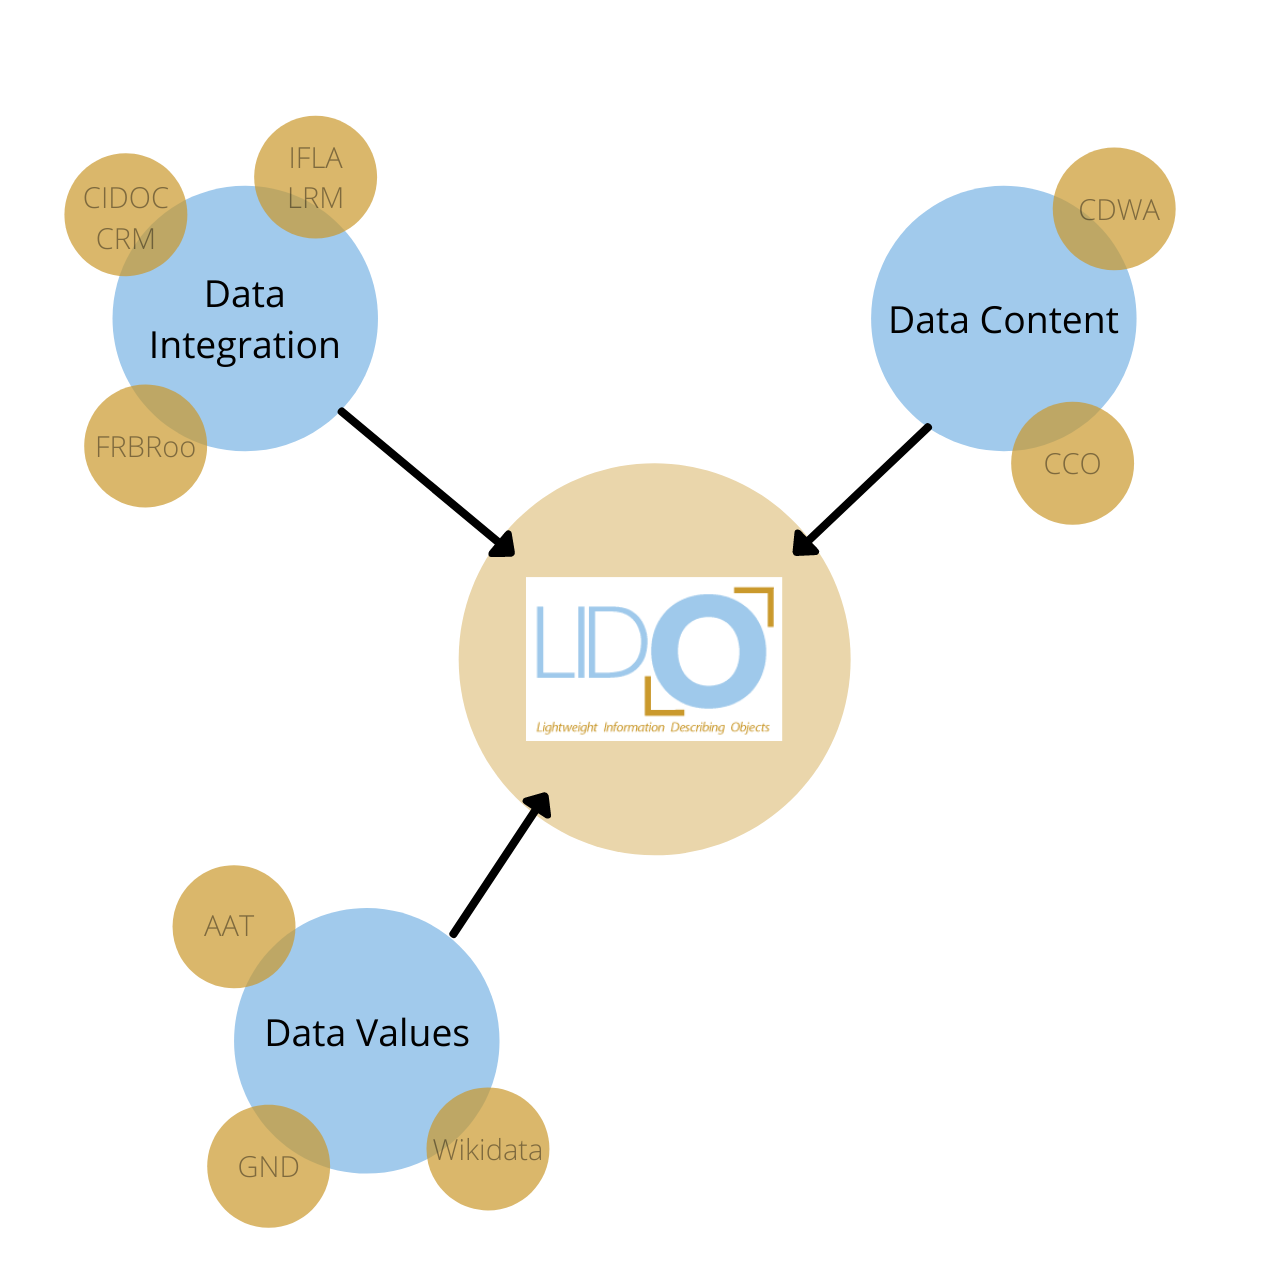
\includegraphics[width=\textwidth]{medias/figure_related-standards.png}}
	\caption{Standards liés au LIDO} 
\end{figure} \newline

Le modèle LIDO a été conçu selon les considérations suivantes :

\begin{itemize}
    \item Réutiliser les normes existantes : Les modèles préexistants de représentation des métadonnées du patrimoine culturel contiennent des propositions qui sont encore valables aujourd'hui. L'ojectif  a été de les réutiliser dans la conception de la LIDO. 
    \item Utiliser des technologies éprouvées : Les métadonnées doivent être traitées dans un large éventail d'environnements système. Le choix de technologies propriétaires ou mal supportées peut entraîner des obstacles et des coûts inutiles.
    \item Faciliter l'interopérabilité  :Les métadonnées sont déplacées, transformées, distribuées et interconnectées à un rythme croissant. Le LIDO devrait donc faciliter et encourager des niveaux d'harmonisation plus élevés que par le passé. Outre les considérations techniques et organisationnelles, les correspondances entre LIDO et les normes ainsi que les modèles d'autres domaines sont des outils essentiels pour permettre et maintenir une telle harmonisation.
    \item Permettre l'adaptabilité :Le paysage de l'information évolue en permanence, faisant apparaître de nouvelles exigences auxquelles il faut répondre sans invalider les enregistrements de données existants. Il faut donc prévoir des adaptation dans le cadre du modèle. En outre, les métadonnées du patrimoine culturel continueront d'être produites à des degrés divers de détail et de granularité. Le modèle doit donc pouvoir s'adapter à des descriptions d'objets d'une richesse très différente en permettant l'introduction de restrictions spécifiques à l'application.
\end{itemize} 
Le choix du XML a été fait en tenant compte tenu de la maturité de celui-ci et de son large soutien dans la sphère du traitement de l'information. Il est possible de penser que cette technologie est et restera une plate-forme solide et fiable pour le schéma de métadonnées du LIDO.\newline

Le langage XML lui-même définit le format des éléments de balisage (souvent appelés balises) et la manière dont ils peuvent être imbriqués pour former une structure arborescente. Tout document XML qui respecte la syntaxe de base des éléments et dont les balises de début et de fin correspondent est dit bien formé.

Pour avoir un traitement prévisible du contenu du document, l'ordre et l'occurrence des éléments de balisage sont généralement limités par un schéma (il s'agit des règle de grammaire du document). Il existe au moins trois langages (DTD, RELAX NG et XSD) permettant d'écrire des définitions de schéma XML. Le schéma LIDO est écrit dans le langage XML Schema Definition (XSD), qui peut être considéré comme le plus expressif de ces trois langages. \newline

La spécification de base du LIDO est définie dans un document XSD. Ce document de schéma peut être utilisé pour vérifier si un enregistrement LIDO est conforme à toutes les règles et restrictions indiquées dans le schéma. Cette validation est essentielle lorsque l'enregistrement LIDO doit être traité pour être utilisé dans des bases de données, des portails web ou dans des chaînes de transformation telles que celles utilisées dans les portails d'agrégation à grande échelle. \footcite{lido_primer}

\begin{figure}[h!]
	\centerline{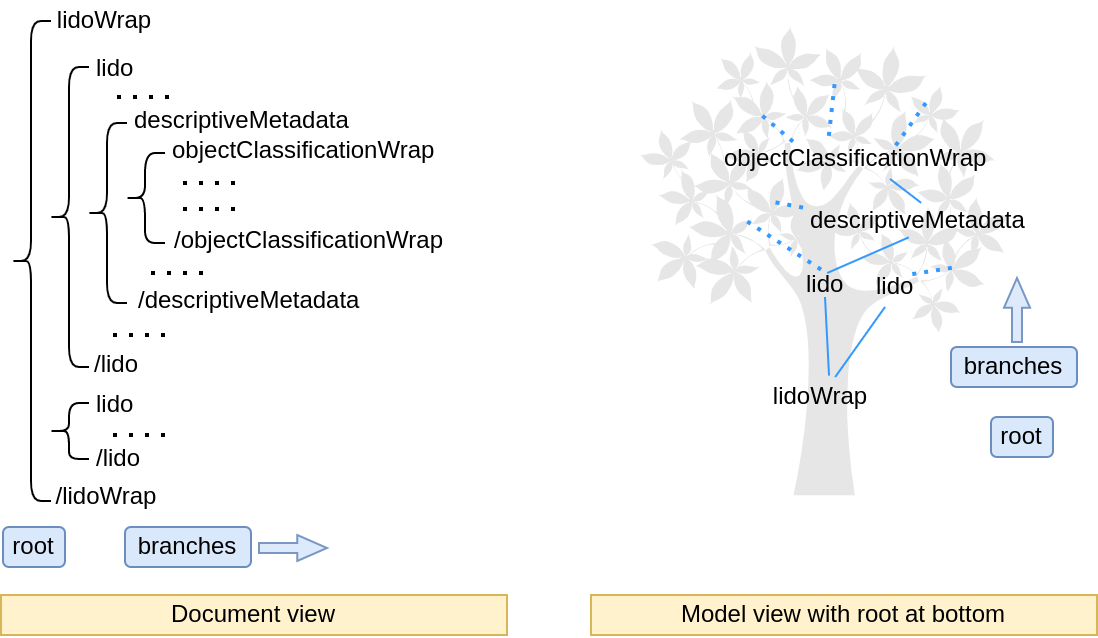
\includegraphics[width=\textwidth]{medias/figure_root-branches.png}}
	\caption{Structure de l'arborescence LIDO} 
\end{figure}